\chapter{Task Resolution}
This chapter will describe all the tasks handled in this sprint in varying degrees of detail depending on the significance and uniqueness of the solution.

\section{Update Dependencies}

This sprint contains three tasks which refer to updating dependencies, the three repositories that we are responsible for updating all require us to update the same three dependencies.
\begin{itemize}
    \item localDB from version 5.1.2 - 5.1.5
    \item meta-database from version 3.2.0 - 3.2.3
    \item oasisLib from version 7.2.0 - 9.0.2
\end{itemize}
\kim{I like that you combined these tasks. However the problem is kind of difficult to understand. Maybe try explainin why you want to update the dependencies. Maybe make some kind of dependency diagram or just illustrate the problem. How many components depend on these?. Also please write a line or two about what localDB, oasisLib, meta-database etc. are.}
As can be inferred by the version numbers updating oasisLib is likely to cause errors as it is two non backwards-compatible versions behind.
localDB and meta-database both pertain to the database where meta-database defines all the tables and keys and localDB pertain to querying the database. 
oasisLib contains models and controllers for said models, updating this particular library causes a variety of errors in the repositories sequence and sequence-viewer.\todo[inline]{Der eksistere ingen dokumentation overhovedet om hvad de 3 depencies er, detter er blot hvad jeg har kunne inferere gennem de methods som er i filerne, what do boys? - M}
\kim{Go search some repports for oasisLib until you find an explanation.}

\begin{description}
    \item[Sequence-Viewer] \hfill \\
    For sequence-viewer updating the oasisLib removes a method being used in order to retrieve pictograms as a new controller for pictograms.
    \kim{There is some information missing here. I am not an expert on android development, but how can pictograms be a controller?  }
    Using the method provided by the new controller provides a nullReference error as the new method for the controller does not work the same as the former method, in order to fix this we explicitly retrieve the name of the pictogram as this is no longer part of retrieving an image and provide a nullcheck, something lacking throughout the system considering the amount of nullReference crashes.
    \kim{This sentence is way to long, add more dots. In the first part of the sentence then you use provided and provides, try not to use the same word twice.  }
    \kim{Instead of saying that it work in a different way, then maybe write the signature of the function. Make the analysis of the problem as precise as possible.}
    \kim{I assume that you also update the dependency to use the newest version, you do not seem to mention this when you descrube your solution.}
    \kim{I dont understand the last part of the sentence.}
    \item[Sequence] \hfill \\
    After upgrading to the newest versions of the libraries mentioned above sequence was unable to build. 
    \kim{Sequence with a captial S please :D}
    This was caused by the usage of a deprecated method. 
    The solution to this issue was fixed by changing a single line to use the correct replacement for the deprecated method.
    \kim{Show me what you canged. I crave code ! ;)}
    The line in question is responsible for loading the pictograms from the database into the application. 
    Previously the model had been used directly however in oasisLib 9.0.2 this is unsupported and one should use the \texttt{pictogramHelper} in the \texttt{Helper}--class, for this operation instead.
    \kim{This sentence is missing some commas. It is not very precise to say that the model was used direcitly, try to describe it more precicly. }
    After this replacement was made then we informally verified that the application worked identically to the previous version with the old dependences
    \kim{missing dot}
    Then a diff was submitted, approved and landed in the master branch. 
    \kim{Is this process that you are refearing to describe somewhere? If not then you properly should.}
\end{description}
\kim{Now you explained the oasisLib problem, what about the other two? }

\subsection{Wiki Migration}
We have the area of responsibility ``Documentation and Wiki'', part of this is ensuring that the information in the Redmine wiki made by the previous GIRAF students is kept since we will depreciate Redmine in favor of Phabricator.
On the Redmine wiki there is a lot of useful information, some of it might be outdated, but most is still useful and should be kept. 

We have taken the task of starting the new wiki on Phabricator, and migrate the useful information from the Redmine wiki to it.
Part of this is to create a structure which the other members of the GIRAF project can use.
It should be noted that the wiki is only used for internal matters inside the GIRAF project.  

It is important that the front page of the wiki is easy to navigate, as this serves as the entry point and from which where all content should be found. 
The contents of the front-page is:

\begin{enumerate}[topsep=0pt,itemsep=-1ex,partopsep=1ex,parsep=1ex]
    \item Actionable Commitments
    \item Guides
    \item GIRAF Project Goals
    \item Useful Links
    \item Sprint Dates
    \item Backlog
    \item Groups and Slack Channels
    \item Wordlist
\end{enumerate}

Most of the content on the wiki are guides which helps the developers with various tasks. 
These should be easy to navigate and have titles which clearly encompass their purpose and content. 
We separate the guides made during this years GIRAF project, which are updated, from the ones made previously. 
Additionally we clearly indicate that the ones constructed previously are not up-to date with the following warning on the top of the page: ``IMPORTANT: This wiki entry has not been updated in 2016''. 

All members of the GIRAF project have access to add to and edit the wiki. 
It is the primary way to share information such as guides and overviews. 
However if this remains unmoderated then the contents of the wiki will most likely become unstructured. 
Therefore in addition the initial migration, we have setup e-mail alerts in Phabricator such that we get a notification every time someone changes the wiki.
Then we will review their additions to ensure that they are located correctly and linked to from the relevant pages etc. 
This will be an ongoing task as part of our area of responsibility.
\section{Consistent File Encoding}
\todo[inline]{TODO}
\section{Responsive Search}
\userstory{As a User I would like the Picto Search application to feel more responsive when I search for pictograms, such that I don't feel like nothing happens.}

The task is prioritised as \phigh,is estimated at 8 EP, and was created because the customers expressed concern for the reactiveness of the PictoSearch application --- it sometimes felt slow and customers said it felt like nothing was happening.
The PictoSearch application is used whenever the user needs to find a certain pictogram for other applications such as the week schedule or the sequence application.
It is a problem that the users feel like the application is slow and that it does not react quickly to what the user is doing, especially in an application used often by other applications of GIRAF.
It is important that responses from a mobile application are given within a few seconds, as mentioned in~\cite{Roto:2005:NNF:1062745.1062747}, if an application spends more than 4 seconds to load or respond then other feedback than visual should be used.
Therefore the amount of time spent waiting for the application should be reduced, such that there is no need for using other methods of feedback when the search finally returns.
According to Constantine and Lockwood in their book \enquote{Software for Use: A Practical Guide to the Models and Methods of Usage-Centered Design} \cite{DESIGNBOOK}, a design principle regarding feedback is as follows:

\begin{displayquote}
\textit{Keep users informed of actions or interpretations, changes of state or condition and errors or exceptions that are relevant and of interest to the user through clear, concise, and unambiguous language familiar to users\cite[p.~57]{DESIGNBOOK}.}
\end{displayquote}

Therefore it is decided that the Picto Search application should give visual feedback whenever an action occurs.
The application should respond to the users action more often than what it does now to increase how responsive the application feels to the user.

The current version of the PictoSearch application searches whenever the user taps the search button on either the on-screen keyboard or in the GUI of the application.
The search button is located in the middle of the screen, to the left of the search field as can be seen on \myref{fig:screenshot_startup}.

\begin{figure}[h]
    \centering
    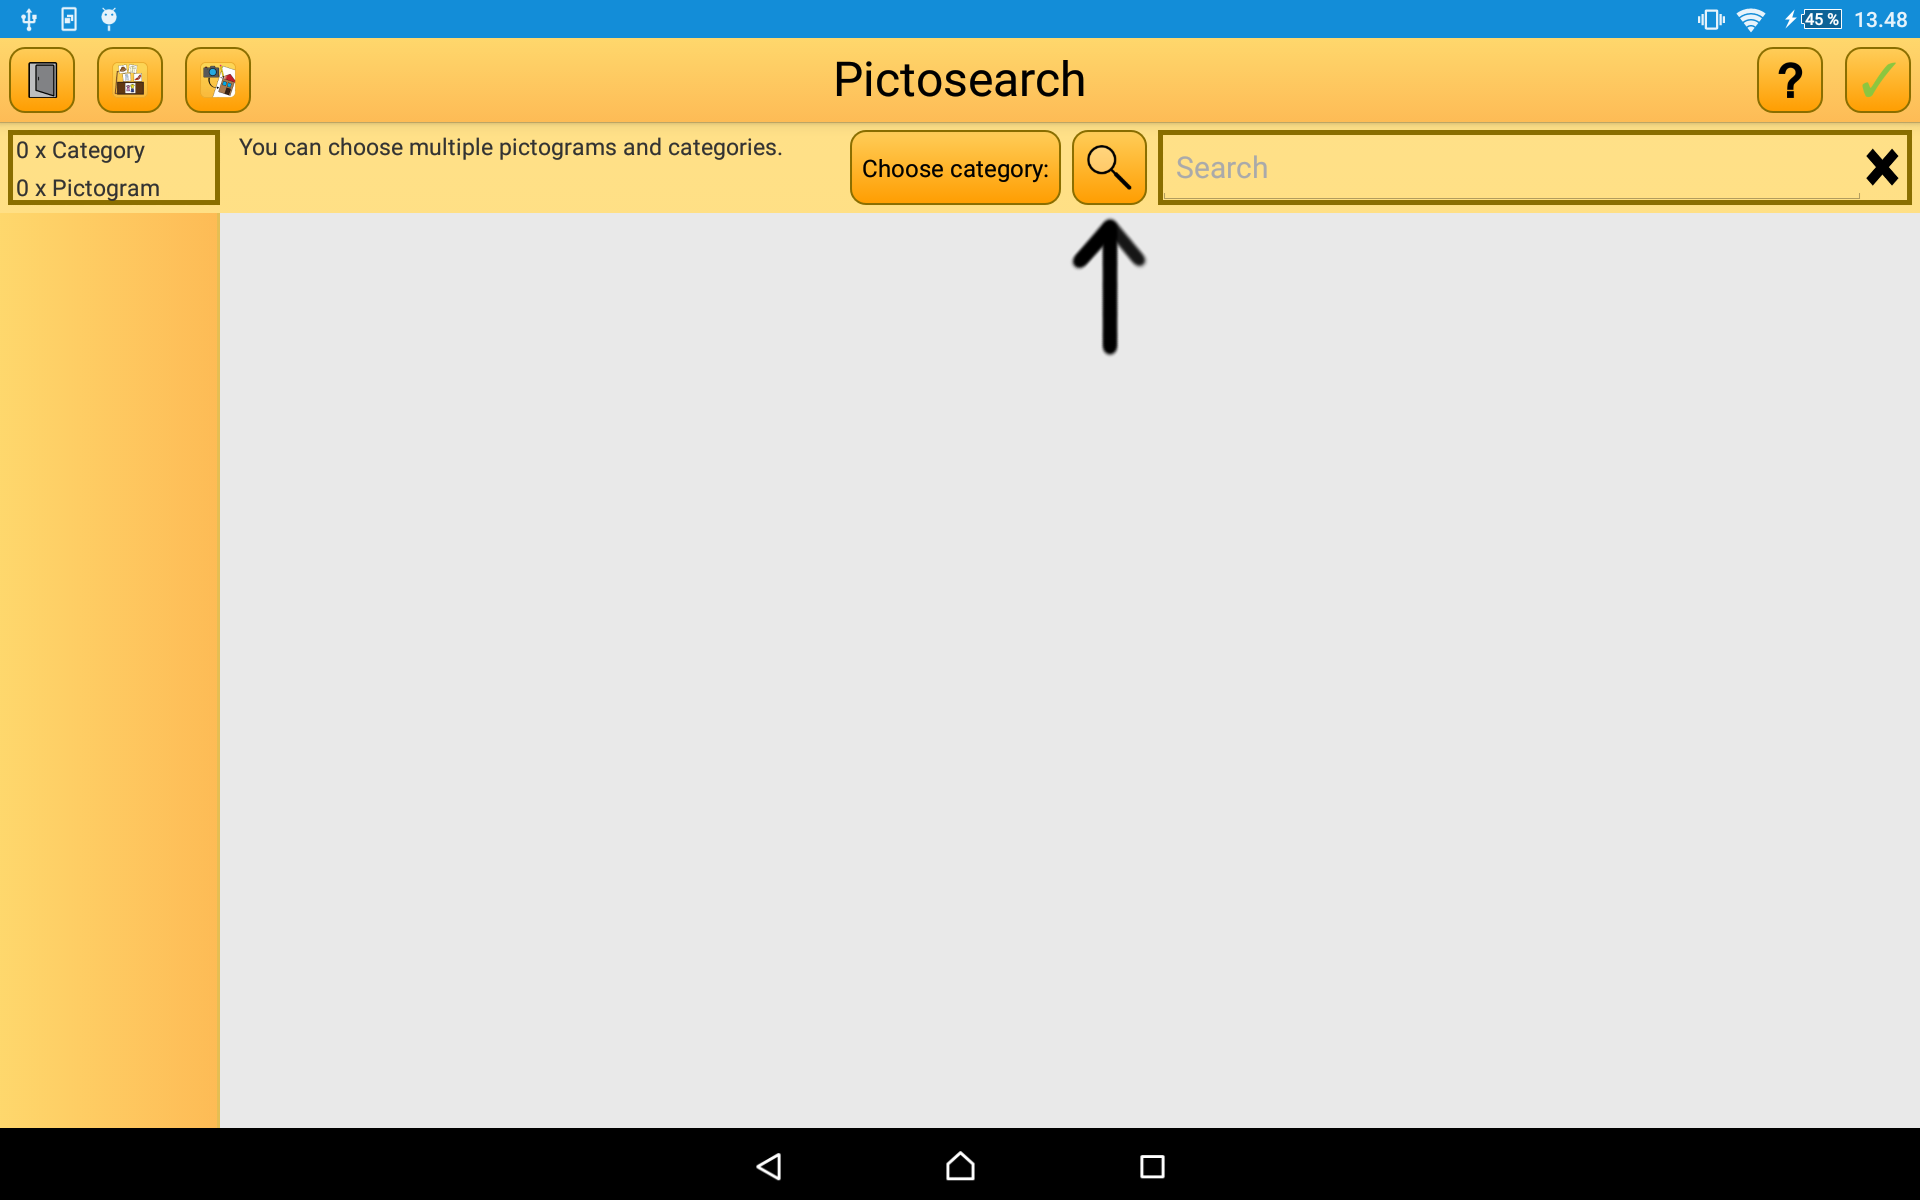
\includegraphics[width=0.8\textwidth]{figures/img/screenshots/old_startup.png}
    \caption{Screenshot of the initial view presented to the user when launching PictoSearch, with the search button highlighted.}\label{fig:screenshot_startup}
\end{figure}
\noindent
The screenshot also shows the view of the application as it is opened, completely empty with no information.

\begin{figure}[h]
    \centering
    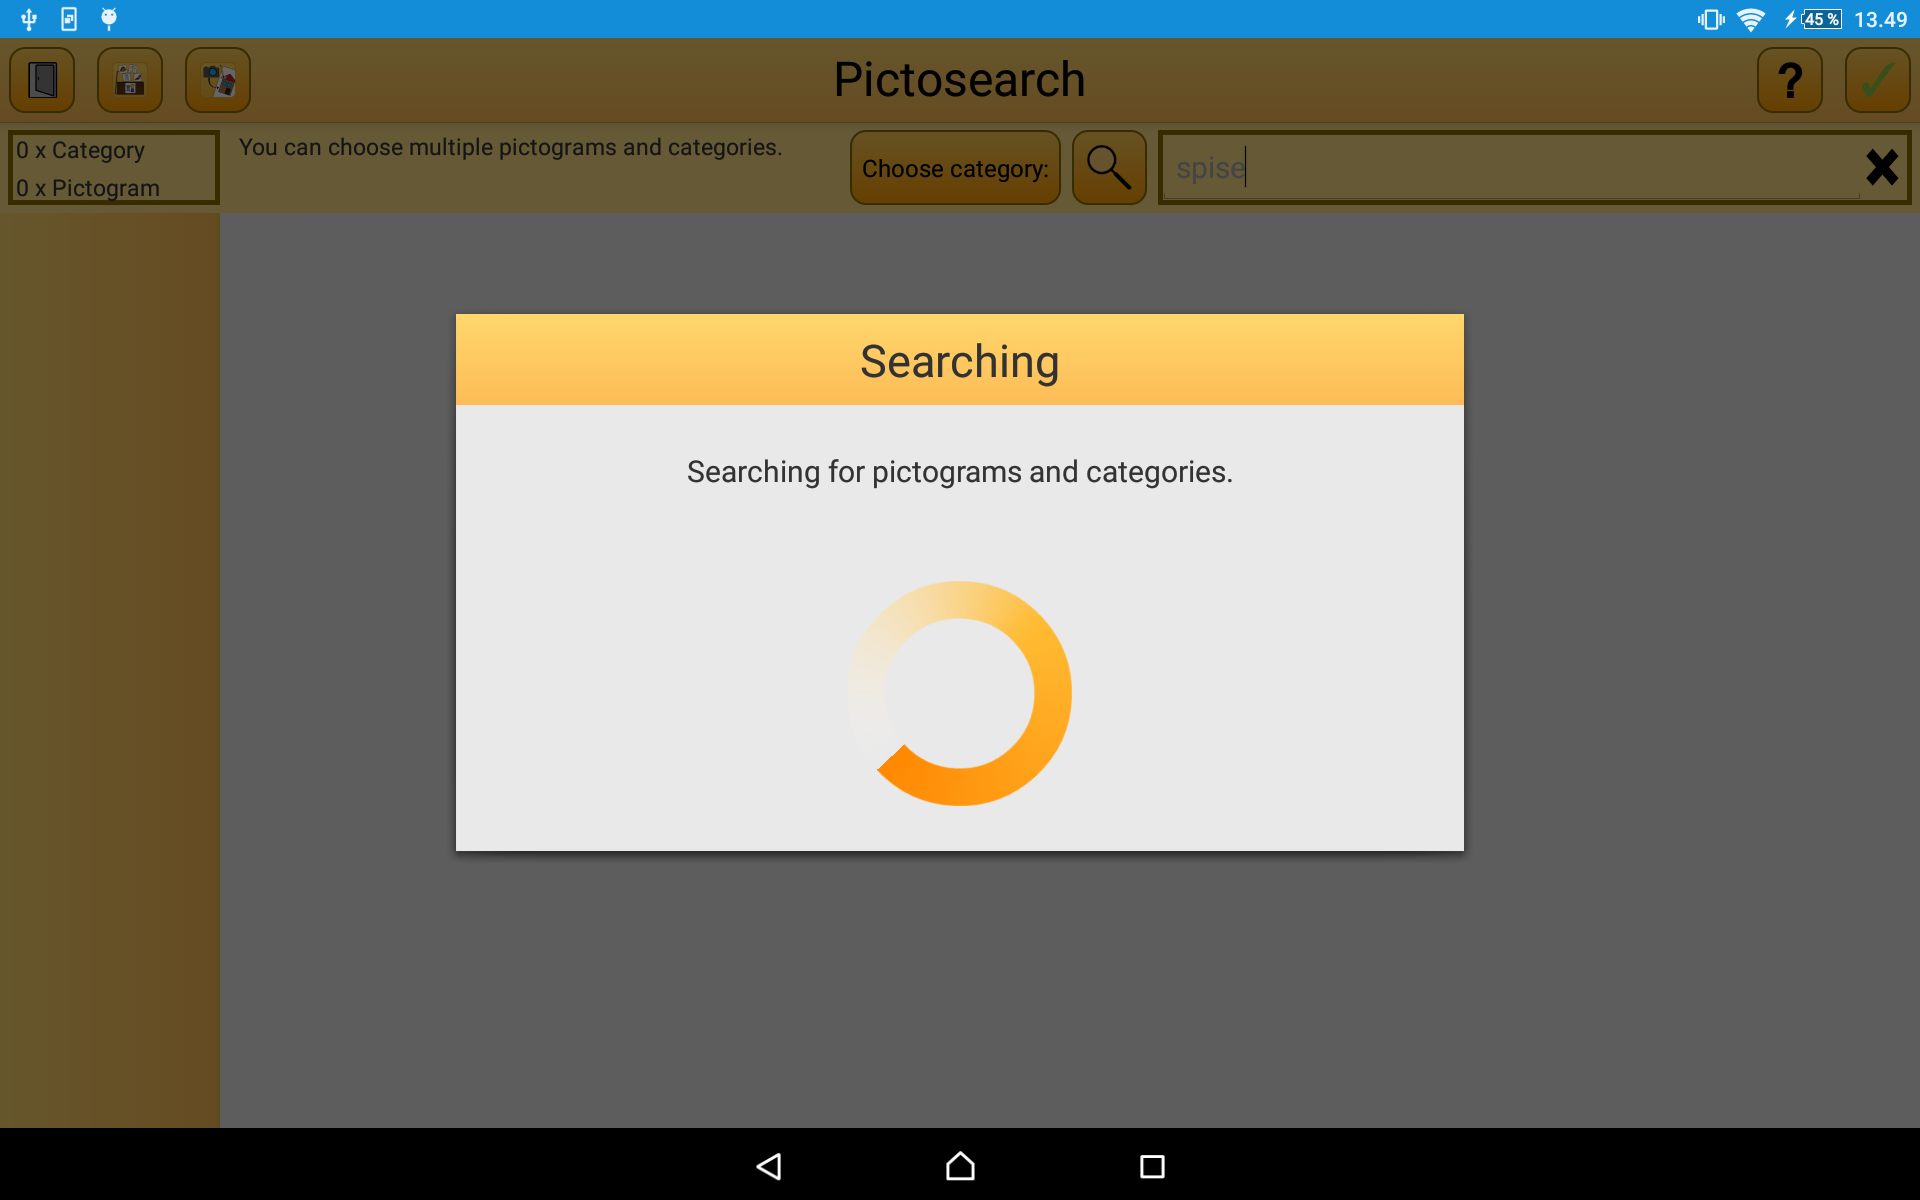
\includegraphics[width=0.8\textwidth]{figures/img/screenshots/old_dialog.png}
    \caption{Screenshot of the search spinner shown while searching in PictoSearch.}\label{fig:screenshot_searchspinner}
\end{figure}

In the new version, a search is made whenever the text in the searchfield is changed.
Instead of the big slow search spinner, which blackened out and locked the screen, shown on \myref{fig:screenshot_searchspinner}, a new smaller text message is instead displayed which tells the user that the application is searching and what is is searching for. 
The current version would also remove the on-screen keyboard when it would search, this only happens in the new version whenever the search button is pressed or the user taps somewhere else, i.e. not on the keyboard.
The application can take input while searching because it is implemented as an async task, i.e. in its own thread.
Because of this any new search is queued behind the current search query, and as such the results of the latest search will be waiting for the results of the previous searches.
This is fixed by a simple change of calling \texttt{AsyncTask.cancel()}, which is a thread.cancellation method, that stops the execution of the ongoing thread and makes it possible to start a new call immediately, with the updated search string, and therefore eliminating the queue.
Because of this anytime a keystroke is made on the keyboard something will happen on the display other than simply filling out the search-field.
When the user types a letter in the textfield, the application will search for the text currently in the text field and display the text as seen on \myref{fig:screenshot_newsearch} explaining what is being searched for. 
This fulfills the principle of giving feedback to the user when an action occurs, such that the user knows what is happening behind the scenes.
When the search returns the pictograms will be shown instead of the text message, with the keyboard still visible.

\begin{figure}[h]
    \centering
    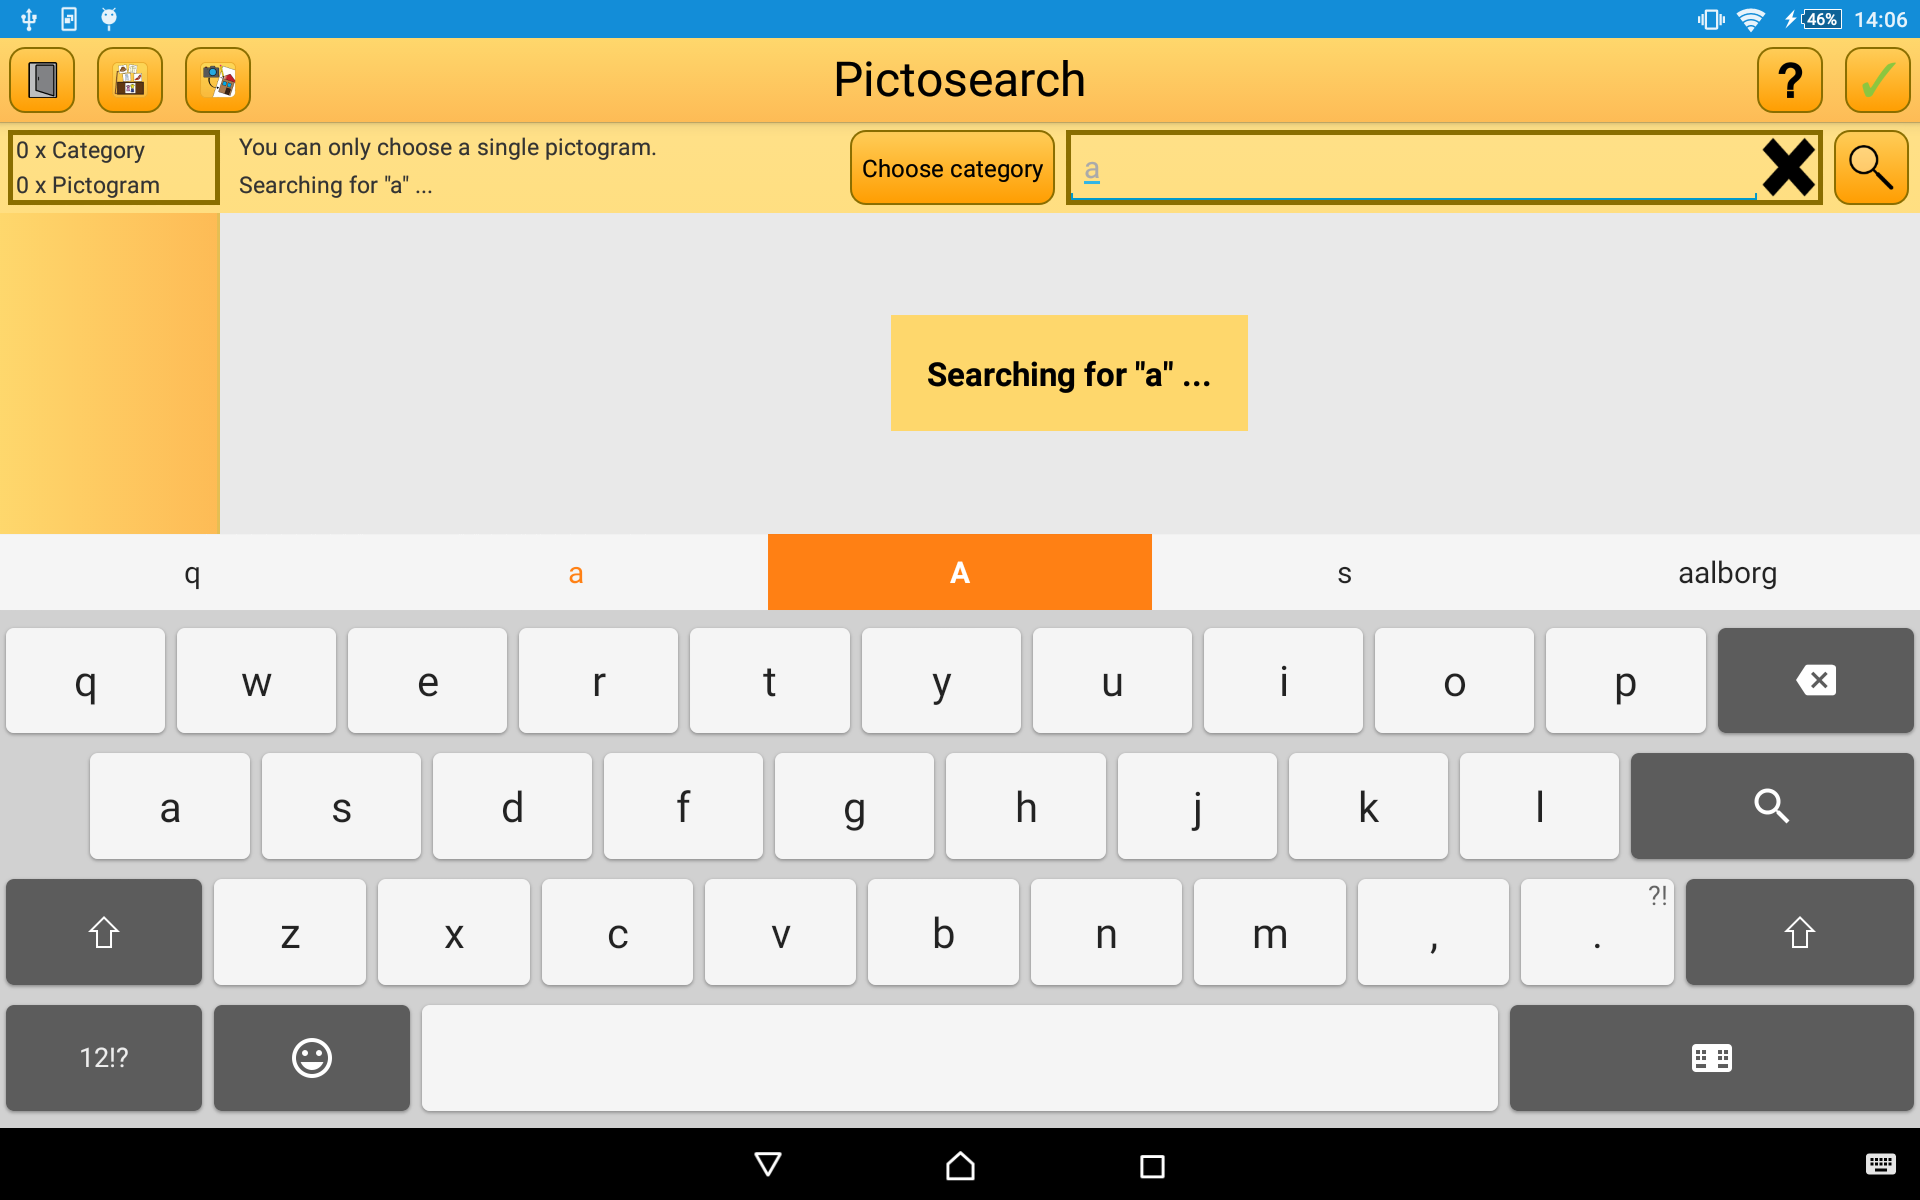
\includegraphics[width=0.8\textwidth]{figures/img/screenshots/new_dialog.png}
    \caption{Screenshot of the new search information, while searching.}\label{fig:screenshot_newsearch}
\end{figure}

This means that there is near instantaneous feedback for the user, which might give the feeling that the application is reacting to whatever the user is doing, and it might no longer feel to users like nothing is happening.
Previously the user would be waiting forever if he thought a search would be performed, when text was entered into the search--field, such as Google does. 
The new approach hereby provides search feedback significantly closer to the aforementioned 4 second limit.
Actually, the query which results in the largest amount of pictograms is a search for the character \enquote{s}, it returns 1932 pictograms and takes approximately 4 seconds on the relatively slow Lenovo tablet provided by the University --- as this is the worst case regarding search time, the average use case will always be faster than 4 seconds. 

The search button can still be used, and will bring up the old search spinner as usually, this is done so that \enquote{refreshing} a search result will provide feedback. 
Moreover the button has been moved from the middle of the display to the right side of the display as can be seen on \myref{fig:screenshot_newstartup}. 
This is a better fit as it resembles other common search engines such as Google Search, and it is also the recommended way to display a search-field according to the Niels Norman Group\footnote{https://www.nngroup.com/articles/magnifying-glass-icon/}.
Furthermore according to the principles of Constantine and Lockwood, structuring the interface is important such that it is for example recognisable: 

\begin{displayquote}
\textit{Organize the user interface purposefully, in meaningful and useful ways based on clear, consistent models that are apparent and recognizable to users, putting related things together and separating unrelated things, differentiating dissimilar things and making similar things resemble one
another.\cite[p.~51]{DESIGNBOOK}.}
\end{displayquote}
\noindent
Therefore using a familiar position of the button is a better fit than placing it in the middle of the screen as in the current version.

Another thing we noticed was that the clear search field button was visible all the time even though no text was in the search field.
This has been removed and it is now only visible when there is text in the search field i.e. when the actoion is available, as can be seen on \myref{fig:screenshot_newstartup} and it it still there on \myref{fig:screenshot_newsearch}.
This has been done because of another design pricinple by Constantine and Lockwood: 

\begin{displayquote}
\textit{Keep all needed options and materials for a given task visible without distracting the user with extraneous or redundant information \cite[p.~55]{DESIGNBOOK}.}
\end{displayquote}

\begin{figure}[h]
    \centering
    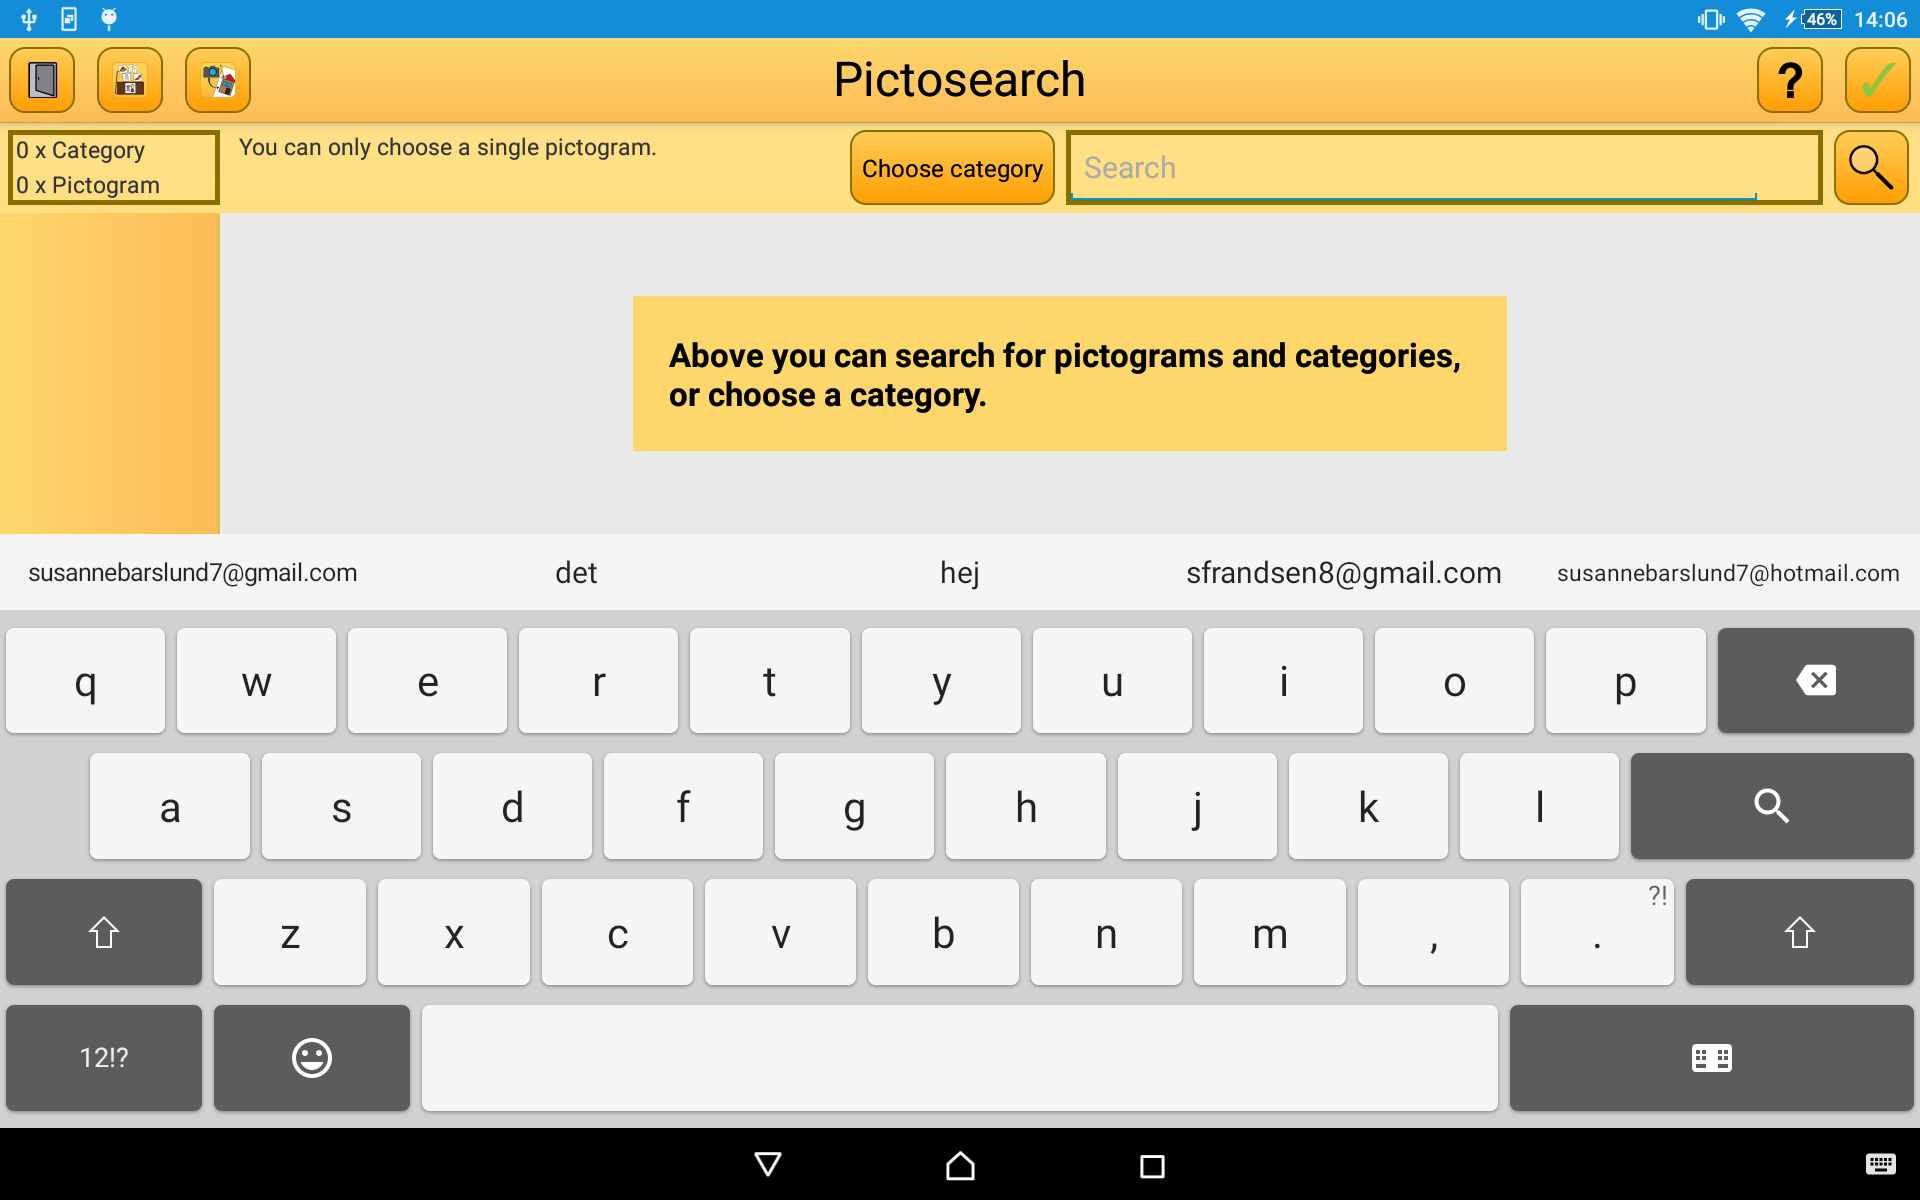
\includegraphics[width=0.8\textwidth]{figures/img/screenshots/new_startup.png}
    \caption{Screenshot of the new initial view in PictoSearch.}\label{fig:screenshot_newstartup}
\end{figure}


\section{dk.giraf.lib Breaks Gradle Build}
\todo[inline]{Nu har vi to rimelig forskellige beskrivelser af hvordan en task er løst, hvilken en vil vi benytte fremadrette? - M}
\section{Sequence wrench should be clickable}
In this section a description of how this high priority task was solved is given, the user story for this task is \textit{As a citizen I want to be able to click on the wrench when editing a sequence, to edit which pictogram is chosen. (Same function as when the picture is clicked)}.
The EP required to solve this task is estimated at N/A as this task was taken on during the sprint in response to us running out of tasks.

\myref{fig:seq_wrench} shows how a guardian using the sequence tool views a sequence, as can be seen there is an image of the sequence thumbnail overlayed with a bin, representing the ability to delete, and a wrench, representing the ability to edit.
The bin indicates that it is deletable, and deletes the sequence if tapped.
The wrench indicates that the sequence can be edited however unlike the bin this does nothing when tapped, despite doing so in other applications where the wrench is used.
When the wrench is tapped it should start the events that are included in editing, as it does if the thumbnail is tapped.
\begin{wrapfigure}{r}{0.3\textwidth}
    \centering
    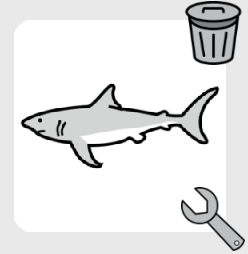
\includegraphics[width=0.3\textwidth]{figures/img/screenshots/sequence_pictogram.png} 
    \caption{A screenshot of a sequence thumbnail as viewed by a guardian.}
    \label{fig:seq_wrench} 
    \vspace{10pt}
\end{wrapfigure}
\bigskip
\noindent
In order to solve this problem firstly we go through the code looking for the implementation of both the bin and the wrench realising that these are both implemented as buttons.
These buttons will henceforth be referred to as the delete and the edit button respectively.
The method \texttt{setupAdapter(final Sequence seq)}, which creates the button view, also calls and overrides the methods that provide their functionality, however no such method is called for the edit button.
An inspection of the code reveals that not only is no such method called, but no such method exists despite the following comment to the method ``\/\/Adds a Delete \& Edit Icon to all Frames which deletes or edits the relevant Frame on click.''.

With the point of failure located a number of solutions present themselves, the fast solution would be to simply write the code as part of the \texttt{setupAdapter} method however this would not be in line with the structure that exists within the sequence code.
Another solution is to find the functionality for when the thumbnail is tabbed and simply copy that, which would be more in line with the structure of the code, yet not be the proper solution.
In order to provide a proper solution which would provide the correct functionality while also maintaining how the rest of sequence has been implemented one could reverse engineer the delete button and use that to construct the proper structure for implementing the edit button.
In order to keep the code maintainable the third option is the solution that we will use, despite knowing it will take more time than the others to implement.

Through further inspection of the code it shows that buttons in sequence are implemented using listeners.
They consist of a handler used to specify the type of click, \texttt{setupOnEditClickHandler()}, an interface with the method \texttt{onEditClick()} and lastly a method, \texttt{setOnEditClickListener(OnEditClickListener listener)}, used to set functionality for the button by overriding \texttt{onEditClick()} when used in order to specify what the button should do at any particular instance.

By creating those three methods and subsequently calling and overriding \texttt{onEditClick()} in the previously mentioned method \texttt{setupAdapter(final Sequence seq)} the issue is fixed without creating any complications.
4 EP is spend on solving the task, mostly on overriding \texttt{onEditClick()} as finding the correct code segments is a lengthy process for while they exist, they were not used until this fix.
